\documentclass[journal]{IEEEtran}
\usepackage{listings}
\usepackage{amssymb}
\usepackage{algpseudocode}
\usepackage{color}

% *** GRAPHICS RELATED PACKAGES ***
%
\ifCLASSINFOpdf
  \usepackage[pdftex]{graphicx}
  
  
\else

\fi

\begin{document}

\title{K-Means Clustering}

\author{Preston Engstrom}
\date{\today}
% make the title area
\maketitle
\lstset{language=Python}

% As a general rule, do not put math, special symbols or citations
% in the abstract or keywords.
\begin{abstract}
The K-Means clustering algorithm has been a mainstay of unsupervised machine learning for decades. The algorithm is explored in this report using known datasets of 2D points, using several cluster counts and distance measures, with results compared using the Dunn Index for cluster analysis.
\end{abstract}


\begin{IEEEkeywords}
Clustering, K-means, Machine Learning
\end{IEEEkeywords}

\IEEEpeerreviewmaketitle


\section{Introduction}
\IEEEPARstart{T}{he} K-Means Clustering Algortihm has continued to be the workhorse of clustering tasks since its development in 1967 by James MacQueen.
In this implementation, the data consists of points on a 2D plain. The clusters are simply the collection of points closest to the center of the cluster based on some distance measure. K-means, and clustering algorithms in general, suffer greatly from the curse of dimensionallity due to their reliance on relating data vectors to each other in a multidimensional space. Presenting data in a 2D space is the best case scenario for exploring the behavior of the algorithm.  The data used in this paper consists of 4 files, S1, S2, S3 and S4. They are ordered in increasing difficulty of clustering, with S1 have the most clearly defined clusters, S4 having the most overlap.

\subsection{Problem Definition}
 Clustering is the task of grouping a set of unlabled data vectors into groups, or clusters. Items in a cluster should be more alike items in the same cluster, and much less like items in other clusters. Clustering is one of the most common tasks of exploratory data mining for extracting preliminary observations about datasets. This paper begins with a description of the K-Means Algorithm and its implementation using the Euclidean, Chebyshev and Minkowski distance measures. The results are then presented and compared using the Dunn Index.



\section{The K-Means Algorithm}
K-Means is a method of vector quantization taken from signal processing. Vector quantization itself is the process of taking a set of complex vectors and compressing them into broader group. With its origins for lossy data compression and lossy error correction, the same processes have been applied for data exploration, pattern recognition and clustering, as in K-Means.

The K-Means alogrithm can be divided into 2 distinct steps. The assignment step and the update step, where the centroids are moved and member data points updated until convergence is reached.



\subsection{Description}
K-Means begins with an initial set of K centroids, wich serve as the centers of each cluster. The assignment step can be expressed as follows[1]:

$$ S_{i}^{(t)} = \{x_{p}: ||x_{p} -m_{i}^{(t)}||^{2 } \leq  ||x_{p} -m_{j}^{(t)}||^{2 } \ \forall j, 1 \leq j \leq k\} $$


Where each data vector $ x_{p} $ is assigned to exactly one cluster $S_{i}$ based on, in the case of this representation, the smallest squared error for each cluster centroid $m_{i} ....m_{j}$. It should be noted that squared error can be expressed as euclidean distance. For each group, the mean of the member data vectors is then calculated, and the clusters centroid is then moved to that position:
$$m_{i}^{t+1} = \frac{1}{|S_{i}^{(t)}|}\Sigma x_{j}$$
This is run for each centroid $x_{j}$. These steps, assignment and update, are repeated until no change occurs between two assignment steps. This convergence generally happens quite quickly, there are points that can extend the running time to $2^{n}$ by preventing convergence even in some cases in 2D[2].

\subsection{Centroid Intialization }
K-Means is a heuristic algorithm and as such cannot guarentee convergence to the global optimum. As such, the algorithm is used with several methods for centroid initialization.


\subsection{Pseudocode Implementation}
\begin{figure}[h]
	
	\caption{Simple K-Means Pseudocode Description}
	\begin{lstlisting}
k_means(k, data_set):
centroids = []
for range(k):
 centroids.add(data_set[k])
change = true
while change:
     for each item in data_set:
       choose the centroid closest
       add item to cluster sum
			
       if current_cluster = last_cluster
   change = false
			
			
	\end{lstlisting}
\end{figure}

\subsection{Distance Measures}
K-Means is built around reducing mean squared error within a cluster. Because we are projecting our data into an n-dimensional space, where $n = |D_{v}|$, where $D_{v}$ is a data vector in our set, it is most common to refer to this measure of error as the mean euclidean distance of points to their centroid. Other distance measures can be used, however the clustering algorithm applied to arbitrary distances is called K-Medoids, not K-means.
\subsection{Euclidean Distance}

The Euclidian distance between two points in 2D P(a,b) and Q(x,y) is defined as:
$$d(P, Q)= \sqrt{(x - a)^{2} +} \overline{(y - b)^{2}}$$

Euclidean Distance is the measure used in the original K-Means. As stated, it is used interchangably as terminology for the mean squared error of a cluster. Minimizing the mean distance of points to a centroid is analogous to reducing the error in our clustering by having points as densly packed as possible around respective means, or more accuratly, to move centroids to the center of distinct groups.
\subsection{Chebyshev Distance}
The Chebyshev distance between two points p and q is defined as:
$$D(p,q):= max(|p_{i}-q_{i}|)$$
Chebyshev distance is also known as chessboard distance. It can be intuitivly explained as follows: The distance between 2 points is the number of moves a king would need to move on a grid to reach one point from the other in 2D. 
\subsection{Minkowski Distance}
The Minkowski Distance of two points x and y is defined as:
$$D(x,y) = (\Sigma|x_{i}-y_{i}|^{p})^{1/p}$$
When $P=1$, it is equivalent to manhatten distance. When p=2, it is equivalent to euclidean distance. The Minkowski distance can also be viewed as a multiple of the power mean of the component-wise differences between $x$ and $y$.
\section{Cluster Analysis Using The Dunn Index}
The Dunn index is a metric for evaluating and comparing the results of clustering algorithms. The Dunn index, and other indexs for clustering result comparison, aim to reward compact clusters which are well separated from neighbouring clusters. For each cluster, the Dunn Index finds the greatest distance between members of that cluster $\textrm{max }\delta(x_{i},y_{i}) $ and the smallest distance between a cluster member and non-member $\textrm{min }  \delta(C_{i}, C_{j})$.
$$DI=\frac{\textrm{min }  \delta(C_{i}, C_{j})}{\textrm{max }\delta(x_{i},y_{i}) }$$
When comparing methods, DI can be used with known data to see how different distance measures can affect results. Where DI becomes more practical is in comparing results for data where the number of clusters is unknown or unclear.
For a range of clusters $[i..n]$, the algoritm can be run a number of times, and the number of clusters with the largest mean DI is selected.

\section{Results and Discussion}
\begin{table}[h]
	\renewcommand{\arraystretch}{1.3}
	
	\caption{Comparison of S-Set Dunn Index, Euclidian Distance}
	\label{table_example}
	\centering
	
	\begin{tabular}{|c|c|c|c|c|}
		\hline
		Dataset & 10 Centroids & 15 Centroids & 20 Centroids & Optimal Value\\
		\hline
		
		S1 & 0.004797  & 0.012200 & 0.005278 & 0.0367893\\
		\hline
		S2 & 0.002901 & 0.005611 & 0.006178 & 0.020947\\
		\hline
		S3 & 0.006027 & 0.008156 & 0.008058 & 0.004394\\
		\hline
		S4 & 0.005708 & 0.006873 & 0.005099 & 0.007474\\
		\hline
	\end{tabular}
\end{table}

\begin{figure}[!t]
\centering
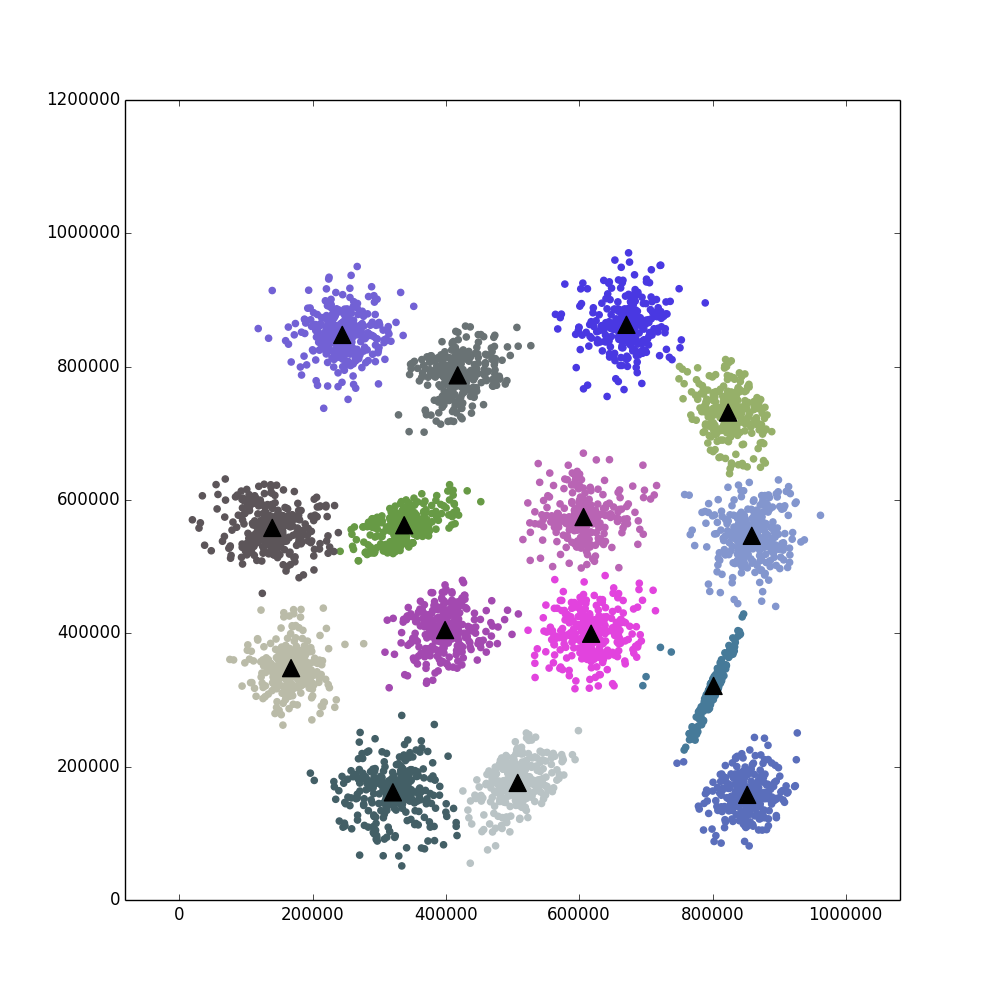
\includegraphics[width=2.5in]{../figs/s1_true_euclid_15.png}
\caption{Optimal Clusters for the S1 dataset.}
\label{fig_sim}
\end{figure}

\begin{figure}[!t]
	\centering
	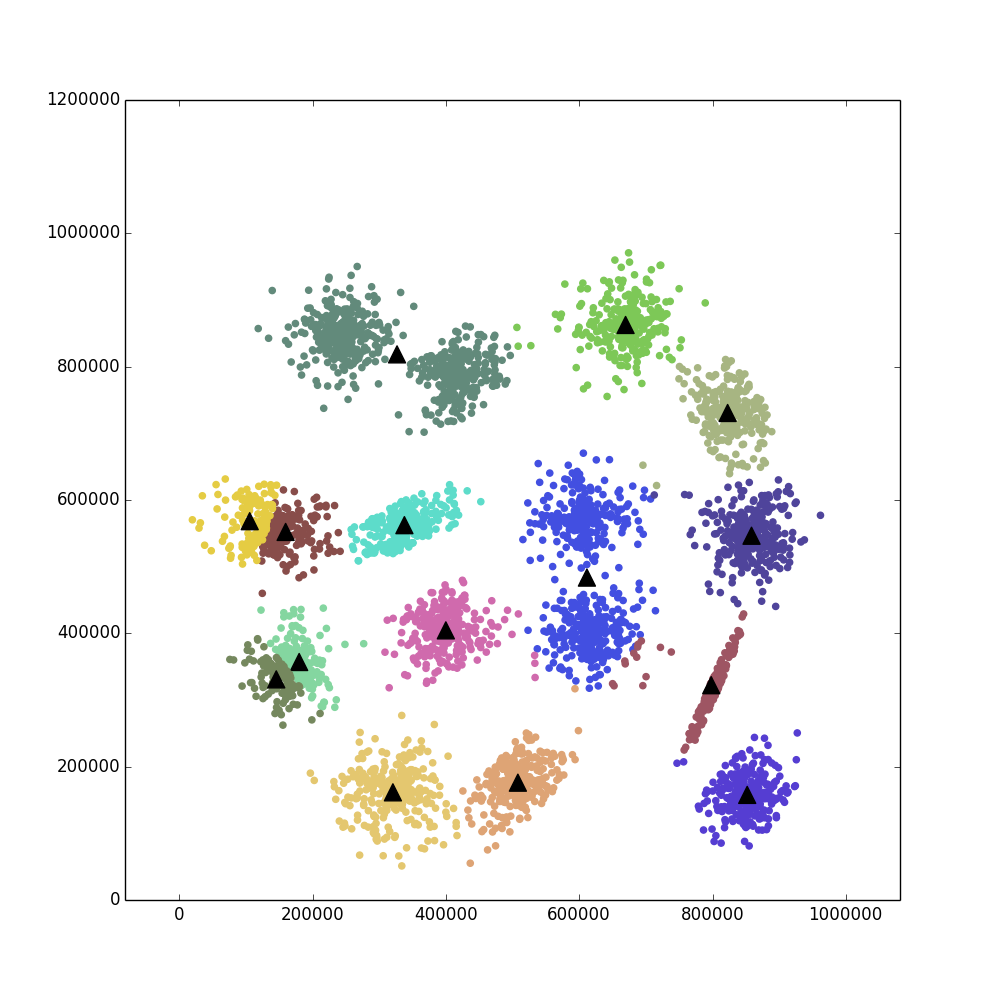
\includegraphics[width=2.5in]{../figs/s1_rand_euclid_15.png}
	\caption{Results using 15 randomly initialized centroids on the S1 Dataset.}
	\label{fig_sim}
\end{figure}

\begin{figure}[!t]
	\centering
	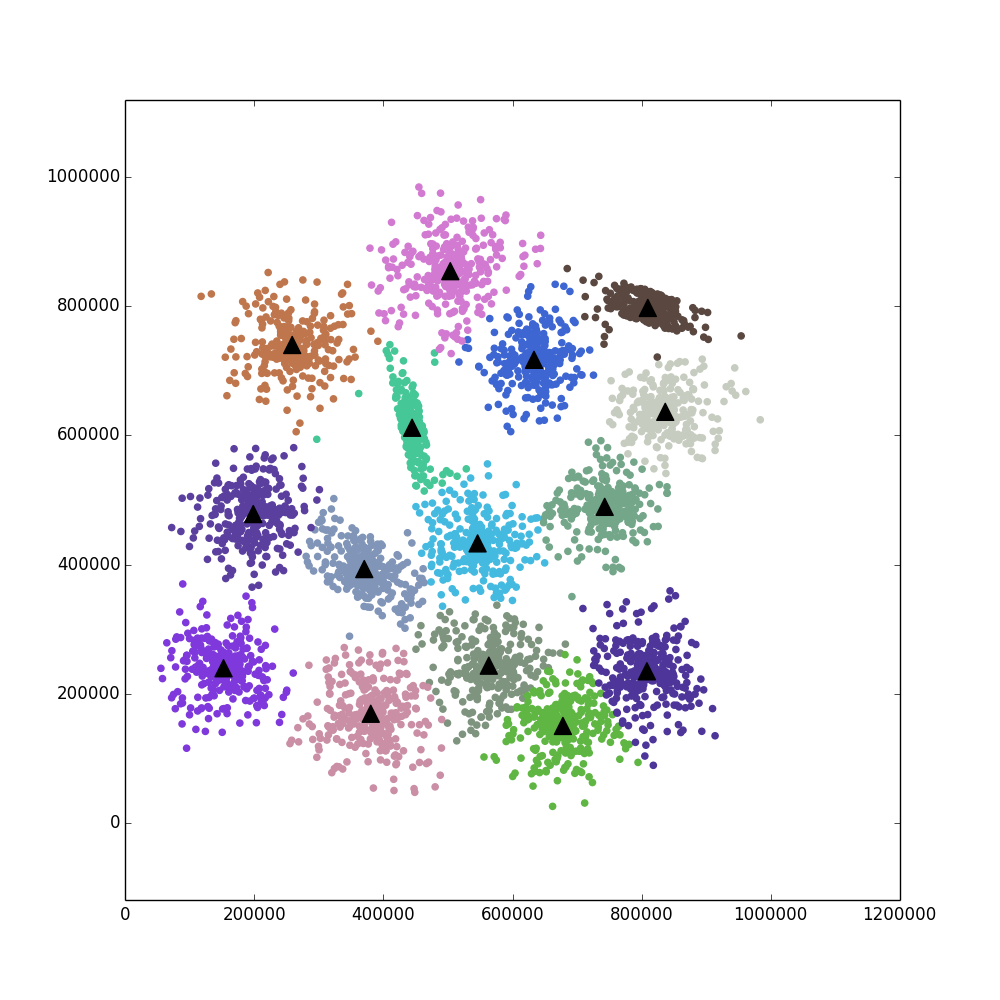
\includegraphics[width=2.5in]{../figs/s2_true_euclid_15.png}
	\caption{Optimal Clusters for the S2 dataset.}
	\label{fig_sim}
\end{figure}


\begin{figure}[!t]
	\centering
	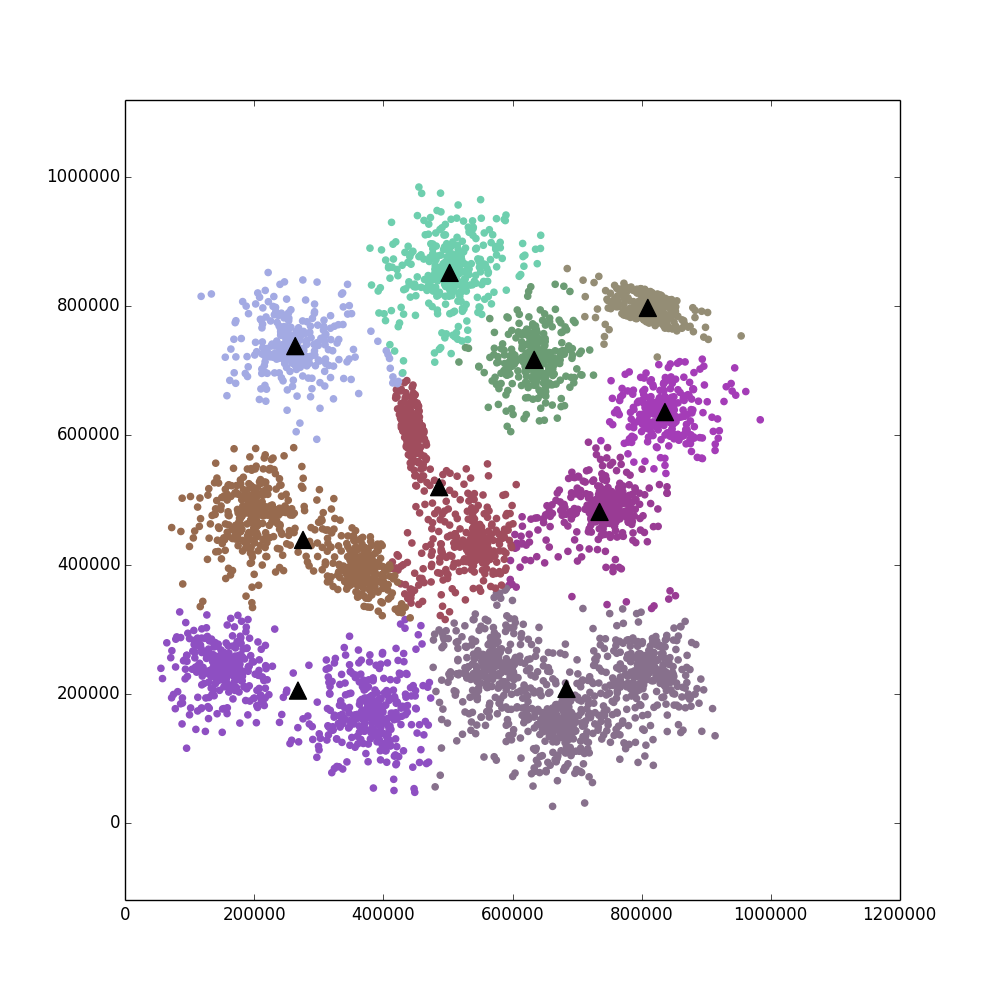
\includegraphics[width=2.5in]{../figs/s2_rand_euclid_10.png}
	\caption{Results using 10 randomly initialized centroids on the S2 Dataset.}
	\label{fig_sim}
\end{figure}

\begin{figure}[!t]
	\centering
	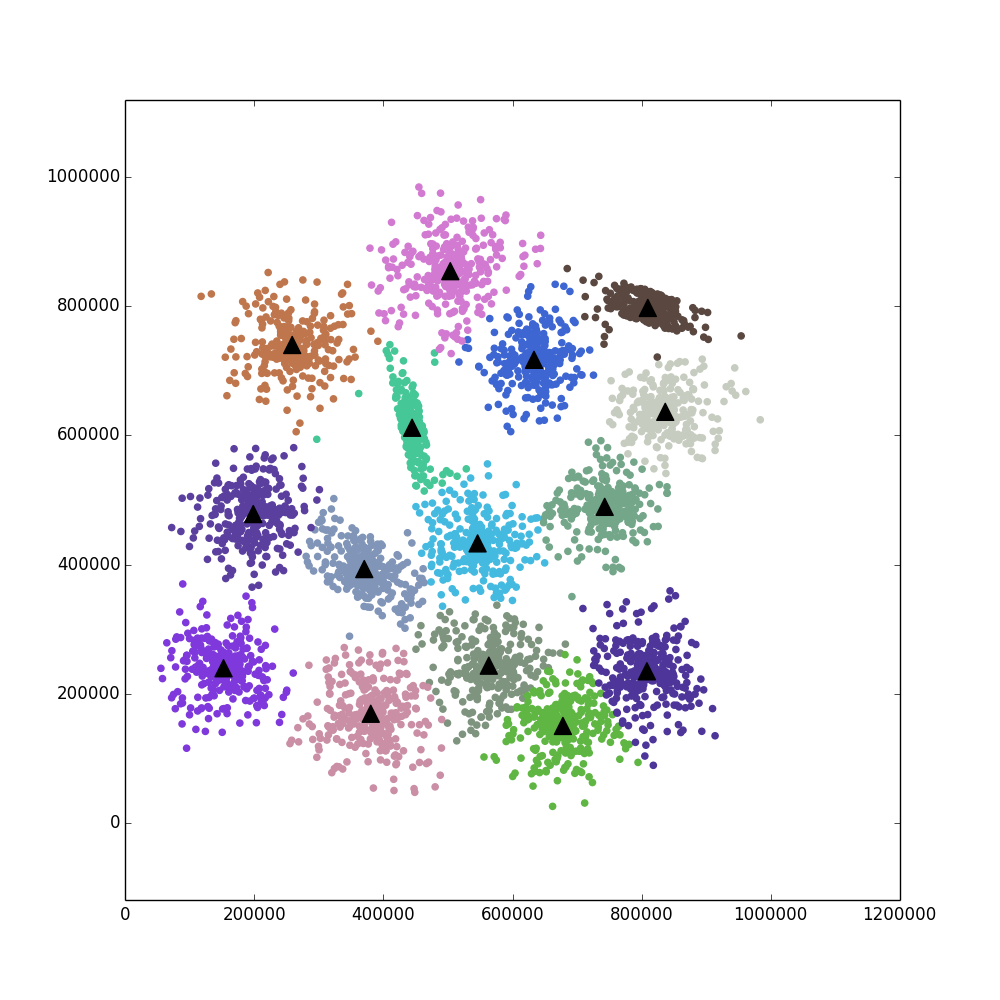
\includegraphics[width=2.5in]{../figs/s2_true_euclid_15.png}
	\caption{Results using Optimal Clusters on the S2 dataset.}
	\label{fig_sim}
\end{figure}
\begin{figure}[!t]
	\centering
	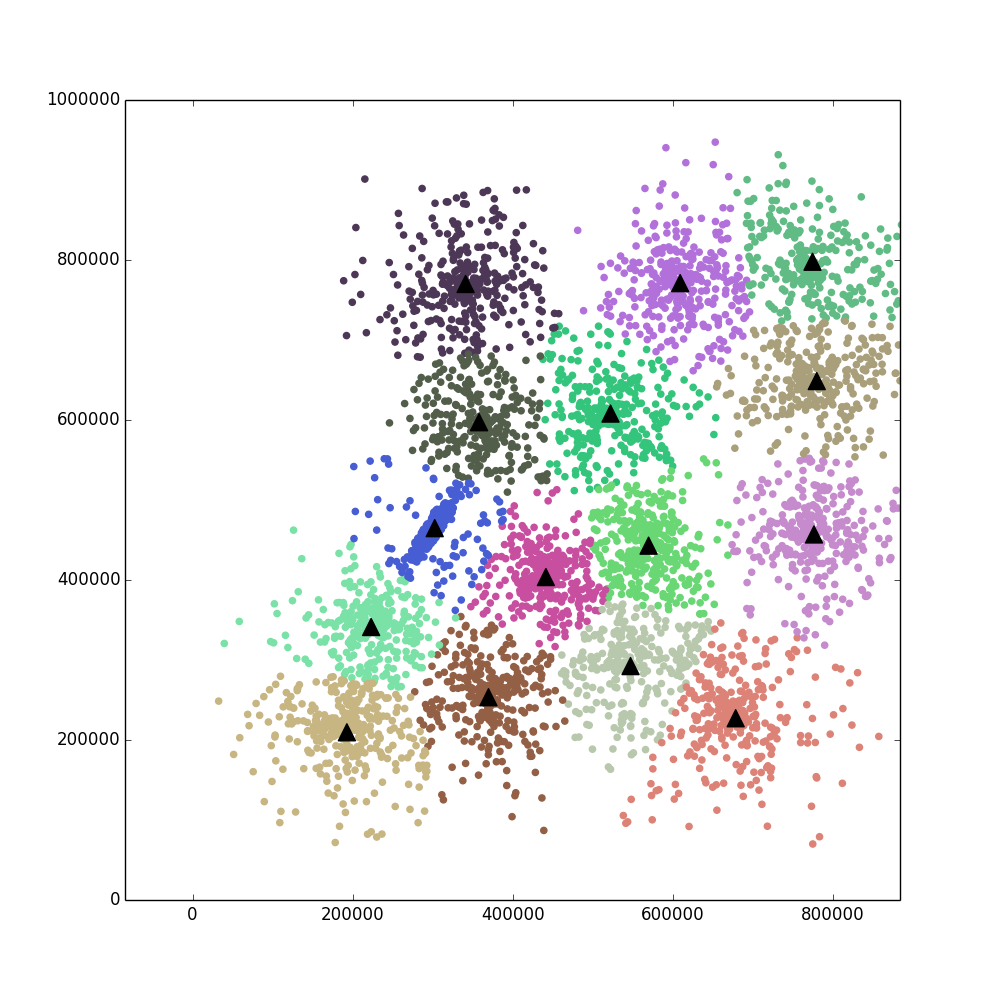
\includegraphics[width=2.5in]{../figs/s3_true_euclid_15.png}
	\caption{Results using Optimal Clusters on the S3 dataset.}
	\label{fig_sim}
\end{figure}
\begin{figure}[!t]
	\centering
	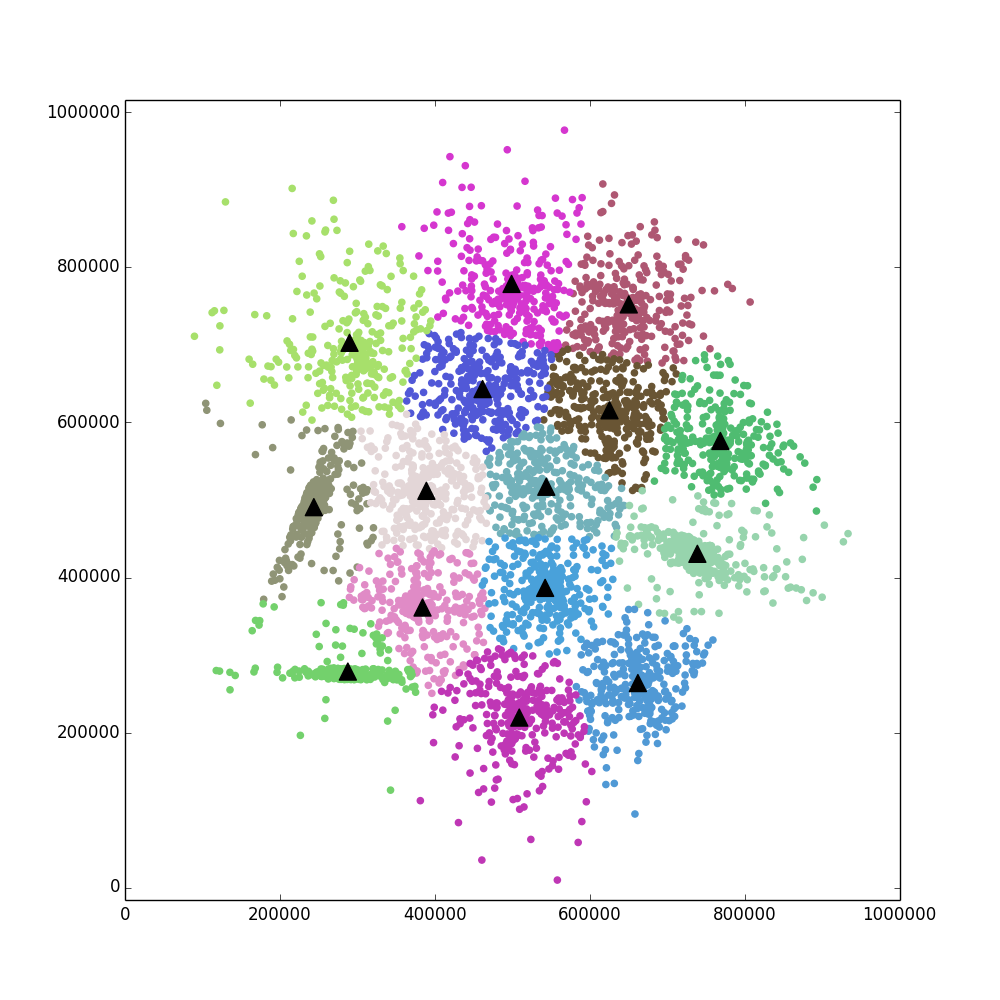
\includegraphics[width=2.5in]{../figs/s4_true_euclid_15.png}
	\caption{Results using Optimal Clusters on the S4 dataset.}
	\label{fig_sim}
\end{figure}



\section{Conclusion}
The experiments perform show that while K-means is a good algorithm for approaching the data clustering problem, the abount of labor involved in reaching a global optimum without prior knowledge of the optimal cluster points in great.

The algorithm and its K-medoids variants will continue to be a mainstay of datamining and machine learning for the forseeable future. They're speed to implement and their ease of analysis and comparison will allow them to remain relevant for years to come.

\ifCLASSOPTIONcaptionsoff
  \newpage
\fi
\begin{thebibliography}{1}
	
	\bibitem{IEEEhowto:kopka}[1]D. MacKay, Information theory, inference, and learning algorithms. Cambridge, UK: Cambridge University Press, 2003.
 \bibitem{IEEEhowto:kopka}[2]A.  Vattani, "k-means Requires Exponentially Many Iterations Even in the Plane", Discrete \& Computational Geometry, vol. 45, no. 4, pp. 596-616, 2011.
\end{thebibliography}



% that's all folks
\end{document}


